\documentclass[12pt]{article}
\usepackage[utf8]{inputenc}
\usepackage{amsmath,amsfonts}
\usepackage{graphicx}
\usepackage{algorithm}
\usepackage{subcaption}

\DeclareMathOperator*{\argmin}{arg\,min}
\providecommand{\m}[1]{\mathbf{#1}}
\providecommand{\norm}[1]{\left\|#1\right\|}
\usepackage{abstract}
\renewcommand{\abstractname}{}    % clear the title
\renewcommand{\absnamepos}{empty} % originally center

\addtolength{\textheight}{1in}
\addtolength{\voffset}{-1in}

\setlength{\textwidth}{5in}
\begin{document}
\title{Auto Scaling Online Learning}
\author{Marco Tulio Ribeiro, Shrainik Jain}
\renewcommand{\today}{Mar 17, 2014}
\maketitle

\begin{abstract}
We propose a framework and algorithms for scaling online machine learning up
or down, according to demand, and the priorities of the system. Different
systems have different needs in terms of the cost assigned to machines, the cost
of a bad user experience, etc. In this project, we focus most on the part that
is general to auto scaling any application (and not only machine learning
algorithms), but propose a framework that takes some ML particularities into
account.
\end{abstract}


\section{Introduction}
Online machine learning algorithms operate on a single instance at a time. They
have become particularly popular in natural language processing and applications
with streaming data, including classification, ranking, etc
\cite{Bordes:2005:HSE:2130928.2130979,
Carvalho:2006:SOL:1150402.1150466, Dredze:2008:CLC:1390156.1390190}. Online
learning is particularly interesting in the scenarios where data keeps streaming
in, such as a web search engine doing advertisement placement. It is also
interesting for scenarios where the whole dataset is too large to fit in main
memory, as online learning only operates on a single example at a time.

A lot of tasks that use online learning have a particular structure that can be 
broken down into 2 major components: 1 - Learning a model from data, and 2 -
making predictions according to the model. Going back to the web search engine
scenario as an example: the system needs to make predictions for every user
doing a query - and must also learn from the feedback given by those users. We
call machines that make predictions \textbf{predictors}, and machines that learn
from the feedback \textbf{learners}.

This structure comes with multiple challenges. First, the 
the amount of data is always growing, so archiving it comes at a cost, both
because of storage constraints and computation constraints. A solution to this
is to just keep the current model in memory, and archive the rest in the
background. A second challenge is the
variable speed at which data streams in. Imagine a learning problem where in the
learning dataset is a live twitter stream for a hashtag. In this scenario the
rate at which the data comes in is a function of the popularity of the hashtag.
Finally, different applications have different costs for learning, and different
requirements for the latency of predictions.

The problem we tackled in this project is the problem of automatically
handling the resources needed for online learning. The ideal system would
allocate the resources necessary to keep the prediction latency acceptable,
while at the same time learning appropriately. Finally, the system would be able
to handle bursts (such as increase in demand) and different learning
requirements for different systems. Since online learning in a distributed
system is a research problem on its \cite{pserver1, pserver2}, we abstracted
this part from our work, and focused on some of the systems challenges.

Current works in auto-scaling\cite{Mao:2011:AMC:2063384.2063449,6008748} address
many of the issues we address in this report (such as load prediction, framing
the problem as a cost minimization problem, etc). However, one aspect that we
thought was lacking in current work (at least from the papers we read) is
dealing with node failures and uncertainty. We reformulate the cost function in
terms of expected cost, in order to account for uncertainty pertaining future
load predictions and node failures. Finally, we evaluate some baselines and our
proposed approach with simulated loads.

\section{Architecture}
\begin{figure}[h!]
\center
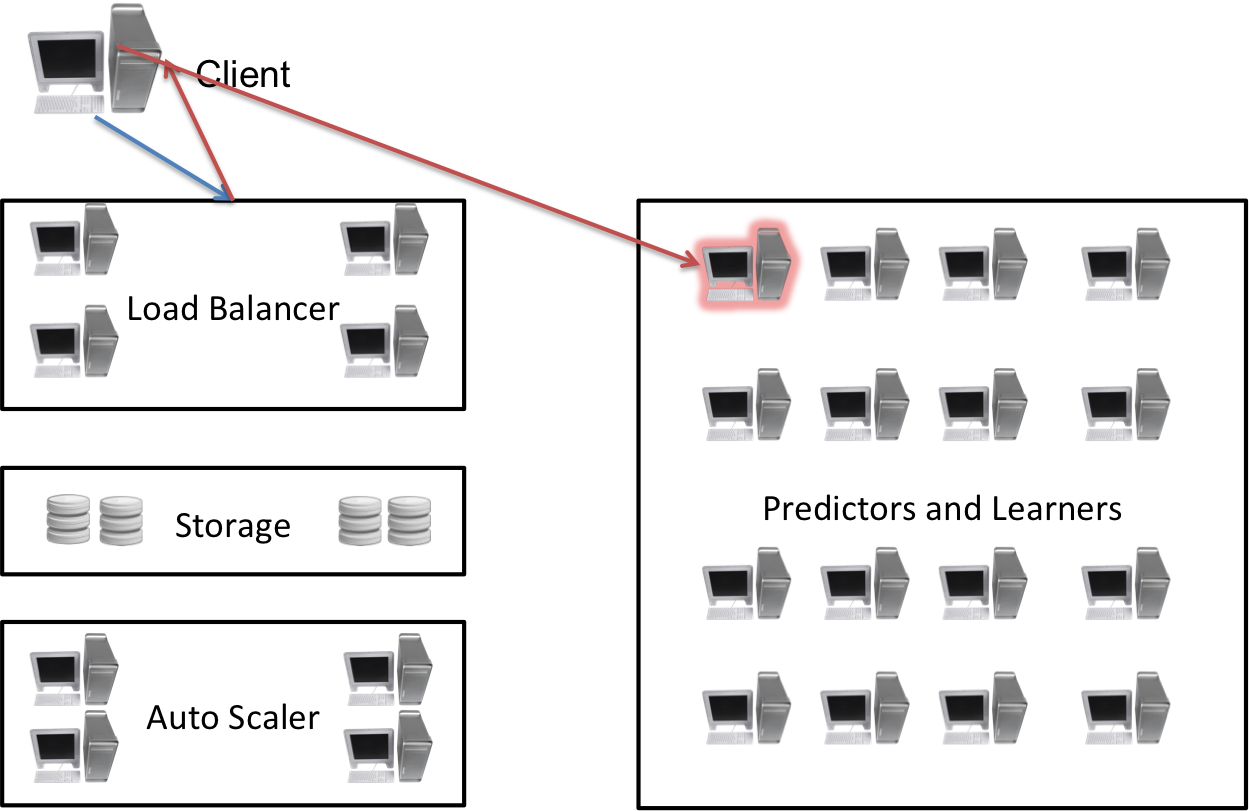
\includegraphics[width=1.0\textwidth]{architecture.png}
\caption{Architecture: Node asks the load balancer for a predictor, and then
asks the predictor for a prediction.}
\label{architecture}
\end{figure}

We assume an architecture similar to the one presented in Figure
\ref{architecture}. There is a set of nodes acting as a Load Balancer
(whose addresses are known to the clients of the machine learning service). When
a client needs a predictor or a learner, it first requests an a node from the
Load Balancer, and then it proceeds to make the request. In Figure
\ref{architecture}, the client got assigned the node in red.

The Load Balancer reads the state of the current system from some distributed,
reliable storage. The state is comprised of which nodes are up and acting as
learners or predictors, and a measure of the \textbf{power} of each node - that
is, how many requests each node can effectively handle in a time interval. This
allows for load balancing even when heterogeneous nodes are present.

The state of the current system is modified every so often by the set of nodes
denoted \textbf{Autoscaler} in Figure \ref{architecture}. The Autoscaler
periodically sends heartbeat messages to nodes and to the load balancer, and
tests the prediction / learning time. It also gets the status - i.e., the number
of requests served, eventual node failures, etc.  Finally, it then updates the
state in the distributed storage according to some policy. This architecture is
very straightforward, and can be used with commodity machines for handling a lot
of requests, while still being resilient to failures (depending of course on the
Autoscaler policy).

\bibliographystyle{plain}
\bibliography{references}

\end{document}
